\chapter{Results}
\section{Problem 1: Simple network}
\section{Problem 2: Backpropagation}
\section{Problem 3: Artificial neural network}
\section{Problem 4: Gradient Descent}

Using the given python code and applying the gradient and weight calculation described in Section~\ref{ch:methods:sec:4} results in the line shown in Figure~\ref{problem4_result}.

The original line is has a $m$ of $3.30$ and a $c$ of $5.3$ and the learned values are $3.28$ for $m$ and $5.27$ for $c$.

\begin{figure}[h]
	\centering
    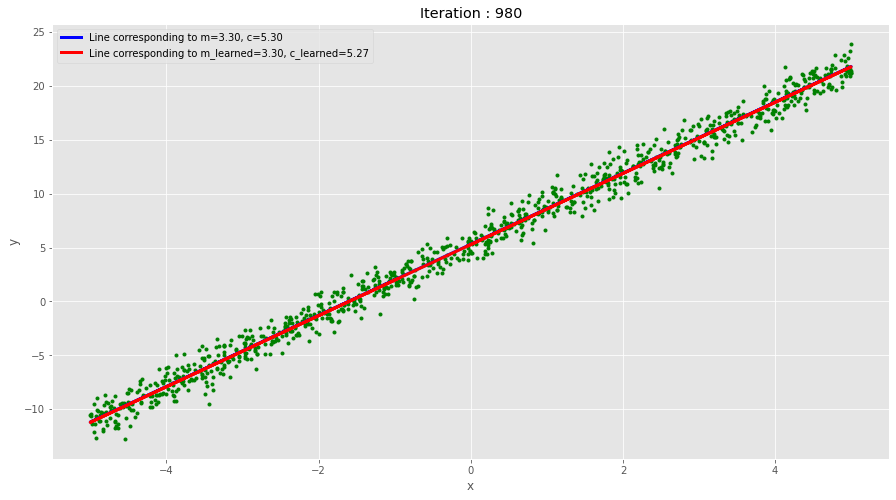
\includegraphics[width=17cm]{img/problem4_result.png}
	\caption{Result of gradient decent}
    \label{problem4_result}
\end{figure}

The loss is also plotted in figure~\ref{problem4_result_loss}.

\begin{figure}[h]
	\centering
    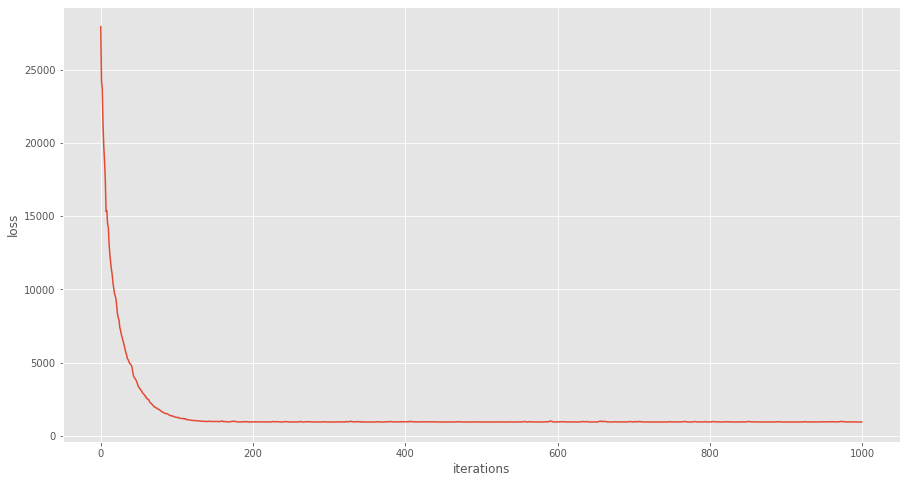
\includegraphics[width=17cm]{img/problem4_result_loss.png}
    \caption{Loss of the gradient decent over the iterations}
    \label{problem4_result_loss}
\end{figure}
